\subsection{Mechanism design}
Now we established all formulas and theories for 2D, 3D and nD-Laplace we are being able to give a full design of the mechanism.

\begin{figure}[H]
    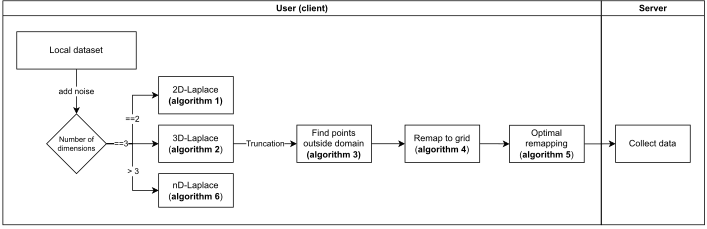
\includegraphics[width=0.6\textwidth]{TheorethicalFramework/ND-Laplace/Images/final_mechanism_design.png}
    \caption{Non-interactive mechanism design for nD-Laplace.}
    \label{fig:final-mechanism-design}
\end{figure}

For easy navigation, we provide a list of all algorithms:
\begin{enumerate}
    \item 2D-Laplace:  \ref{alg:2d-laplace}
    \item 3D-Laplace: \ref{alg:3d-laplace}
    \item nD-Laplace: \ref{alg:nd-laplace}
    \item Find points outside domain: \ref{alg:find-outside-domain-laplace}
    \item Grid remapping: \ref{alg:grid-remapping-laplace}
    \item Optimal remapping: \ref{alg:optimal-remapping-laplace}
\end{enumerate}